
\documentclass{standalone}
\usepackage{tikz}
\usepackage{amsfonts}

  %
  \usepackage{tikz} %
  \usetikzlibrary{
	petri, %
	backgrounds, %
	arrows, %
	positioning, %
	decorations.markings, %
	calc,  %
	fit, %
  }
\def\backgrnd{black!20}	% Background for Tikz pictures
\pgfdeclarelayer{edgelayer}
\pgfdeclarelayer{nodelayer}
\pgfdeclarelayer{background}
\pgfsetlayers{background, edgelayer,nodelayer,main}
\tikzstyle{place}=
[circle,thick,draw=blue!75,fill=blue!20,minimum size=6mm]
\tikzstyle{antiplace}=
[circle,thick,draw=red!75,fill=red!20,minimum size=6mm]
\tikzstyle{transition}=
[rectangle,thick,draw=black!75,fill=black!20,minimum size=4mm]
\tikzstyle{inarrow}=[->, >=stealth, shorten >=.03cm,line width=0.5]
\tikzstyle{outarrow}=[<-, >=stealth, shorten <=.03cm,line width=1.5]

\tikzset{
	pics/netA/.style args={#1/#2/#3/#4/#5/#6/#7}{code={
					% \fill[yellow!15] (-0.8,-2.3) rectangle (2.3, 2.3);

					\node [place,label=above:$p_1$, tokens={%
								#1
							}] (-pl_1) {};

					\node [transition,label=above:$t$, label=below:#5] (-tr_1) [right = of -pl_1] {};

					\node [place,label=above:$p_2$, tokens={%
								#2
							}] (-pl_2) [right = of -tr_1] {};

					\node [transition,label=left:$v$, label=above:#6] (-tr_2) [below = of -tr_1] {};
					\node [transition,label=below:$u$, label=above:#7] (-tr_3) [below = of -tr_2] {};

					\node [place,label=below:$p_3$, tokens={%
								#3
							}] (-pl_3) [left = of -tr_3] {};

					\node [place,label=below:$p_4$, tokens={%
								#4
							}] (-pl_4) [right = of -tr_3] {};

					\draw[inarrow] (-pl_1) -- (-tr_1);
					\draw[inarrow] (-tr_1) -- (-pl_2);
					\draw[inarrow] (-pl_2) -- (-tr_2);
					\draw[inarrow] (-tr_2) -- (-pl_3);
					\draw[inarrow] (-tr_2) -- (-pl_4);
					\draw[inarrow] (-pl_3) -- (-tr_3);
					\draw[inarrow] (-tr_3) -- (-pl_4);
				}}
}


  %
  \tikzset{ %
		oriented WD/.style={%
			every to/.style={
        out=0,in=180,draw
      },
			label/.style={
				font=\everymath\expandafter{\the\everymath\scriptstyle},
				inner sep=0pt,
        node distance=2pt and -2pt
      },
			semithick,
			node distance=1 and 1,
			decoration={
        markings, mark=at position \stringdecpos with \stringdec
      },
			ar/.style={
        postaction={decorate}
      },
			execute at begin picture={
        \tikzset{
					x=\bbx, y=\bby,
					every fit/.style={
            inner xsep=\bbx, inner ysep=\bby
          }
        }
      }
		},
		string decoration/.store in=\stringdec,
		string decoration={
      \arrow{stealth};
    },
		string decoration pos/.store in=\stringdecpos,
		string decoration pos=.7,
		bbx/.store in=\bbx,
		bbx = 1.5cm,
		bby/.store in=\bby,
		bby = 1.5ex,
		bb port sep/.store in=\bbportsep,
		bb port sep=1.5,
		bb port length/.store in=\bbportlen,
		bb port length=4pt,
		bb penetrate/.store in=\bbpenetrate,
		bb penetrate=0,
		bb min width/.store in=\bbminwidth,
		bb min width=1cm,
		bb rounded corners/.store in=\bbcorners,
		bb rounded corners=2pt,
		bb small/.style={
      bb port sep=1, 
      bb port length=2.5pt, 
      bbx=.4cm, bb min width=.4cm, 
      bby=.7ex
    },
		bb medium/.style={
      bb port sep=1, 
      bb port length=2.5pt, 
      bbx=.4cm, 
      bb min width=.4cm, 
      bby=.9ex
    },
		bb/.code 2 args={%
			\pgfmathsetlengthmacro{\bbheight}{\bbportsep * (max(#1,#2)+1) * \bby}
			\pgfkeysalso{
        draw,
        minimum height=\bbheight,
        minimum width=\bbminwidth,
        outer sep=0pt,
        rounded corners=\bbcorners,
        thick,
				prefix after command={
          \pgfextra{\let\fixname\tikzlastnode}
        },
				append after command={
          \pgfextra{
            \draw
            \ifnum #1=0
              {} 
            \else 
              foreach \i in {1,...,#1} {
						  	($(\fixname.north west)!{\i/(#1+1)}!(\fixname.south west)$) +(-
							\bbportlen,0) 
              coordinate (\fixname_in\i) -- +(\bbpenetrate,0) coordinate (\fixname_in\i')
              }
            \fi 
						%
            \ifnum 
              #2=0{} 
            \else 
              foreach \i in {1,...,#2} {
							($(\fixname.north east)!{\i/(#2+1)}!(\fixname.south east)$) +(-
							\bbpenetrate,0) 
              coordinate (\fixname_out\i') -- +(\bbportlen,0) coordinate (\fixname_out\i)
              }
            \fi;
          }
        }
      }
		},
		bb name/.style={
      append after command={
        \pgfextra{
          \node[anchor=north] at (\fixname.north) {#1}
        ;}
      }
    }
	}




\begin{document}
\scalebox{3}{
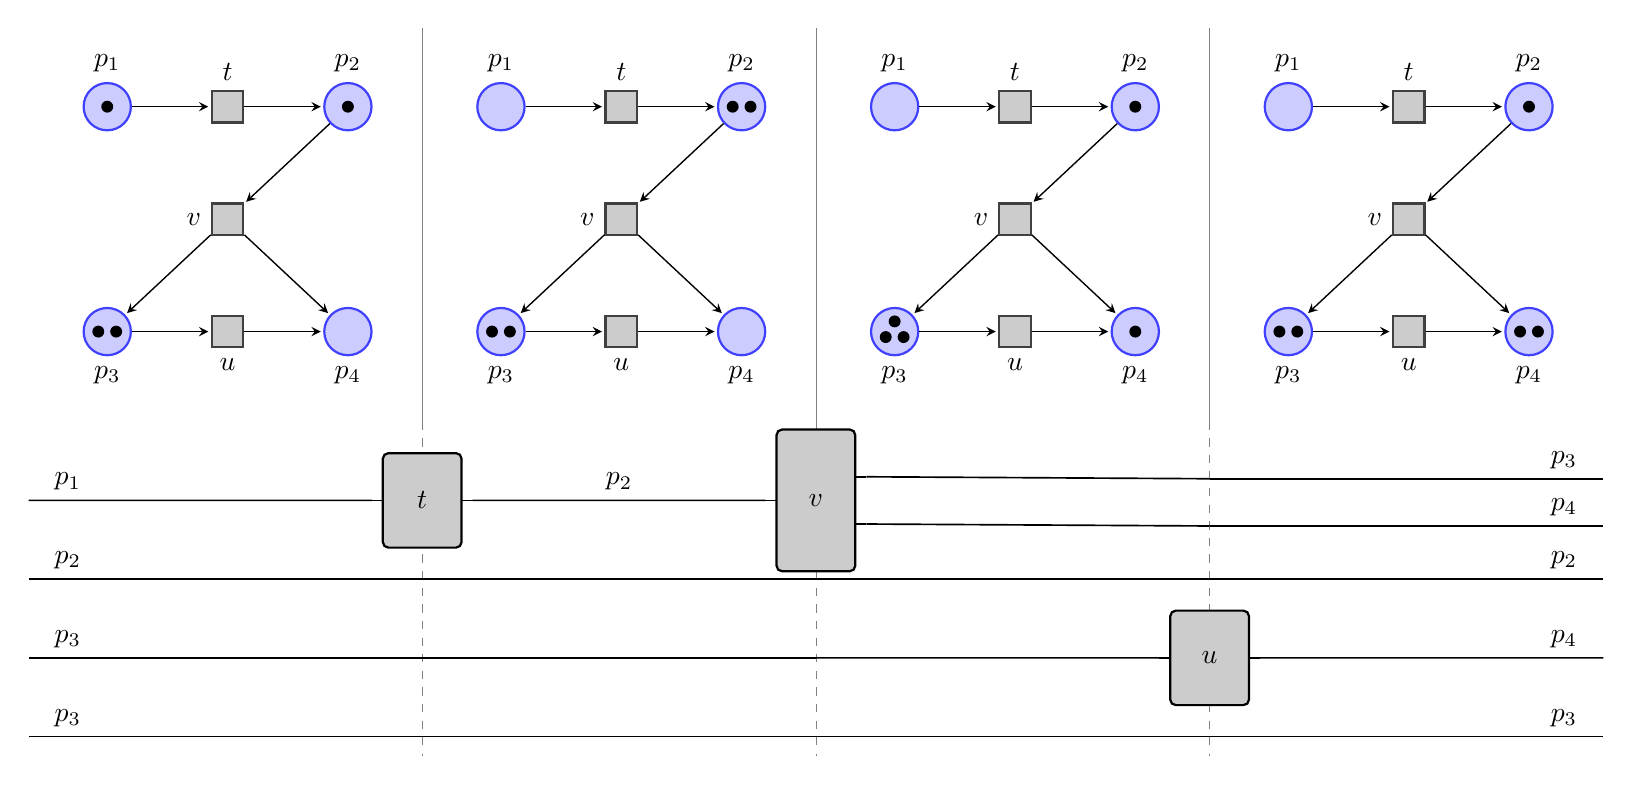
\begin{tikzpicture}
	\pgfmathsetmacro\bS{5}
	\pgfmathsetmacro\hkX{(\bS/3.5)}
	\pgfmathsetmacro\kY{-1.5}
	\pgfmathsetmacro\hkY{\kY*0.5}
	\draw pic (m0) at (0,0) {netA={{1}/{1}/{2}/{0}/{}/{}/{}}};
	\draw pic (m1) at (\bS,0) {netA={{0}/{2}/{2}/{0}/{}/{}/{}}};
	\draw pic (m2) at ({2 * \bS},0) {netA={{0}/{1}/{3}/{1}/{}/{}/{}}};
	\draw pic (m3) at ({3 * \bS},0) {netA={{0}/{1}/{2}/{2}/{}/{}/{}}};
	\begin{scope}[very thin]
	\foreach \j in {1,...,3} {
			\pgfmathsetmacro \k { \j * \bS - 1 };
			\draw[gray,dashed] (\k,-4) -- (\k,-8.25);
			\draw[gray] (\k,1) -- (\k,-4);
		}
	\end{scope}
	\begin{scope}[shift={(0,-4)}, oriented WD, bbx = 1cm, bby =.4cm, bb min width=1cm, bb port sep=1.5]
		\draw node [fill=\backgrnd,bb={1}{1}] (Tau) at (\bS -1,-1) {$t$};
		\draw node [fill=\backgrnd,bb={1}{2}, ] (Mu)  at ({2 * \bS - 1},-1) {$v$};
		\draw node [fill=\backgrnd,bb={1}{1}] (Nu)  at ({3 * \bS - 1},{2 * \kY}) {$u$};
		\draw (-1,-1) --     node[above] {$p_1$}       (0,-1)
		--                  node[above] {}          (Tau_in1);
		\draw (-1,-2) -- node[above] {$p_2$} (0,-2) -- (\bS-1, -2);
		\draw (-1,-3) -- node[above] {$p_3$} (0,-3) -- (\bS-1, -3);
		\draw (-1,-4) -- node[above] {$p_3$} (0,-4) -- (\bS-1, -4);
		\draw (Tau_out1) -- node[above] {$p_2$}    (Mu_in1);
		\draw (\bS-1,-2) -- (2*\bS-1, -2);
		\draw (\bS-1,-3) -- (2*\bS-1, -3);
		\draw (\bS-1,-4) -- (2*\bS-1, -4);
		\draw (Mu_out1) --  (3*\bS-1, -0.725);
		\draw (Mu_out2) --  (3*\bS-1, -1.325);
		\draw (2*\bS-1,-2) -- (3*\bS-1, -2);
		\draw (2*\bS-1,-3) -- (Nu_in1);
		\draw (2*\bS-1,-4) -- (3*\bS-1, -4);
		\draw (3*\bS-1,-0.725) to (4*\bS-2, -0.725) -- node[above] {$p_3$} (4*\bS-1, -0.725);
		\draw (3*\bS-1,-1.325) -- (3*\bS,-1.325) to (4*\bS-2, -1.325) -- node[above] {$p_4$} (4*\bS-1, -1.325);
		\draw (3*\bS-1,-2) to (4*\bS-2, -2) -- node[above] {$p_2$} (4*\bS-1, -2);
		\draw (Nu_out1) to (4*\bS-2, -3) -- node[above] {$p_4$} (4*\bS-1, -3);
		\draw (3*\bS-1,-4) to (4*\bS-2, -4) -- node[above] {$p_3$} (4*\bS-1, -4);
	\end{scope}
\end{tikzpicture}
}{}


\end{document}